\chapter{Technical Background}
In this chapter we delve into the technical details underpinning
the security of \ac{TLS} and \ac{ECH},
as well as the principles we will leverage in desiging \ac{SECH}.

\section{The One-Time Pad}
In this section we'll try to give a somewhat technical and somewhat intuitive explanation as to how and why stream-cipher based encryption works,
in particular why the bits of a well constructed ciphertext should give an eavesdropper no information about the bits of the associated plaintext,
and why the ciphertext is
difficult to distinguish from true
uniform random values.

To keep things simple let's assume Alice wants to send Bob a message $m$ consisting of one bit, either 0 or 1, over an insecure channel.
And we assume that Alice has announced publicly that she will send the message to Bob
at some specified time, i.e. the fact of sending the message is not confidential.
An eavesdropping attacker wants to gain information about which value Alice is sending to Bob, whether it is 0 or 1.
The attacker may already have correct prior knowledge about the probability of each value,
e.g. that Alice has a 25\% chance of sending a 0 and a 75\% chance of sending a 1.
In this case, without even looking at an encrypted message, the attacker already believes with 75\% certainty that Alice's message will be 1.
Alice and Bob's goal is to ensure that the eavesdropping attacker does not update its belief based on observations of the encrypted message,
i.e. that the attacker does not {\em gain} any information about the message.

The \ac{OTP} provides a mechanism to achieve this `perfectly', in the sense that
the attacker will gain no information.
Let's assume Alice and Bob each have a copy of a \ac{OTP} $k$ of length 1 bit.
In general each bit of a \ac{OTP} must be sampled as a fair coin, 50\% chance of 0 and 50\% chance of 1.
To create the ciphertext $ct$ we simply perform the element-wise \ac{XOR} operation between $m$ and $k$.
For Alice's single bit message this results in the below probabilities in Table~\ref{otp-xor-probs-example} assuming the prior 25/75 distribution of $m$.
If the eavesdropper observes $ct=0$ then the posterior distribution of $m$ is still $P(m=0)=0.125/0.5=0.25$ and $P(m=1)=0.375/0.5=0.75$.
The distribution has not changed and the attacker has gained no information.
This holds generally regardless of the prior distribution.
Notice also the related fact that $P(ct=0)=P(ct=1)=0.5$.

\begin{table}[H]
\centering
\begin{tabular}{llllll}
$m$ & & $k$ & & $ct$ & $P$    \\
0 &  $\oplus$  & 0 & = & 0    & 12.5\% \\
0 & $\oplus$  & 1 & = & 1    & 12.5\% \\
1 & $\oplus$  & 0 & = & 1    & 37.5\% \\
1 &  $\oplus$  & 1 &= & 0    & 37.5\%
\end{tabular}
  \captionsetup{width=.8\linewidth}
\caption[Probabilities after XOR with Random Key]{\label{otp-xor-probs-example}For a secret one bit message $m$ with prior probabilities $P(m=1)=0.75$ and $P(m=0)=0.25$ and a secret \ac{OTP} $k$, the probabilites of each combination, $P(m,k)$, as well as the ciphertext attained by $m\lxor k$ are listed.}
\end{table}

For other binary operators such as the \ac{lAND} the distribution of $ct$ is different as we see in Table~\ref{otp-and-probs-example}. For \ac{lAND} we get $P(ct=0)=0.625$. This means that if the eavesdropper observes $ct=0$ then the posterior distribution of $m$ is inferred as $P(m=0)=0.25/0.625=0.4$ and $P(m=1)=0.375/0.625=0.6$, and this distribution is different from the prior distribution meaning that information was gained!

\begin{table}[H]
\centering
\begin{tabular}{llllll}
$m$ & & $k$ & & $ct$ & $P$    \\
0 &  $\land$  & 0 & = & 0    & 12.5\% \\
0 & $\land$  & 1 & = & 0    & 12.5\% \\
1 & $\land$  & 0 & = & 0    & 37.5\% \\
1 &  $\land$  & 1 &= & 1    & 37.5\%
\end{tabular}
  \captionsetup{width=.8\linewidth}
\caption[Probabilities after AND with Random Key]{\label{otp-and-probs-example}For a one bit message $m$ with prior probabilities $P(m=1)=0.75$ and $P(m=0)=0.25$, the probability of each possible configuration is listed. We end up with a lower entropy distribution of $ct$ than for \ac{XOR}, with $P(ct=0)=0.625$ and $P(ct=1)=0.375$.}
\end{table}

It turns out that \ac{XOR} and its negation are the only two binary operators that give us a uniform distribution of $ct$ when using a uniformly distributed $k$. Thus we can construct a perfect crypto system assuming the \ac{OTP} $k$ can be securely shared between Alice and Bob. For some problems this solution is practical, e.g. if a military field operative knows they will be sending a top secret message back to base they can securely share the \ac{OTP} at the base and use it later when in the field. However, the requirement for the two parties to securely share $k$ ahead of time makes the use of a true \ac{OTP} impractical in most cases. The principle, though, of \ac{XOR}ing the message $m$ with a (pseudo)random key $k$ is a central component of modern symmetric crypto systems.

Under the assumption that $k$'s bits are truly random we get the result that $m\lxor k$ is indistinguishable from true randomness. This property of the ciphertext being indistinguishable from random values is the basis on which we will build our approach to a stealthy \ac{SNI}/\ac{ALPN} encryption scheme. However, instead of using truly random keys we will use pseudorandom key streams to approximate a truly random \ac{OTP}. A good pseudorandom key stream has bits which are drawn from a very close approximation of the uniform distribution over ${0,1}$. Any deviations in a pseudorandom key stream's distribution from the uniform distribution will also be reflected in $ct$, and $ct$ will thus be theoretically distinguishable from true randomness, given enough samples. However, if the pseudorandom stream's distribution is close enough to the true uniform distribution, then distinguishing the ciphertext from true random data will be practically infeasible.

\section{Cryptographic Hash Functions}
A hash function is a function that maps arbitrary length data to a fixed length representation. An example of a (completely useless) hash function is the function that maps all inputs to the 0x00 byte. Useful hash functions often approximate a uniform distribution over the possible outputs for different inputs. If a hash function has an output length of one byte (256 possible outputs), and we feed in random strings to the hash function, it is desirable (for many use cases) if each of the 256 possibilities are approximately equally represented in the outputs. Hash functions with this property are useful in designing efficient algorithms and data structures (e.g. hash tables). However, the uniform distribution of outputs is not a sufficient property for making the hash function a secure cryptographic hash function. It is possible that the output of such a hash function reveals some information about the input.

Let's construct an example of a hash function whose output reveals information about the input, we interpret the input message as an unsigned integer (with an arbitrary number of bits) and take the modulo of this integer and the number of possible outputs (256). Therefore the messages "0x00", "0x01", "0x02", ..., "0xFF" are all mapped to themselves, so we get a perfect uniform distribution for all one-byte messages. In fact, any message is just mapped to the least significant byte of the message, and therefore, the hash output tells us deterministically what the last byte of the message was.

For hash functions used in cryptographic algorithms this is not acceptable; we need hash functions where the hash digest (output) reveals nothing about the input message. Our insecure last-byte hash function is fast to compute (it's $O(1)$, just take the last byte), but it turns out that cryptographically secure hash algorithms are more compute intensive because they digest the entire input message (they are at least $O(N)$). One might not want to use a cryptographic hash function for non-cryptographic tasks (efficient lookup, hash tables etc.) because they may be more compute-intensive than non-cryptographic alternatives.

Cryptographic hash functions must, of course, be deterministic, i.e. for the same input it always returns the same output.
This property is essential for the use of cryptographic hash functions for integrity checks. In a communications setting,
like \ac{TLS}, integrity checks are performed by sending a message alongside the cryptographic hash of the message.
The receiver can verify that the message and hash match with each other, which provides assurance that
the message was not modified.
Non-cryptographic hash functions can be useful for integrity checks when the threat model does not include an
intelligent active attacker. E.g. if the threat model is just that random modification may occur due to hardware glitches,
then a deterministic non-cryptographic hash function may be appropriate.
However,
when the threat model includes communication over an insecure channel when an active attacker can tamper with messages,
determinism is not sufficient for the security of integrity checks.

A preimage attack on a hash function is one where an attacker attempts to find an input $m$ which produces a particular output $\text{\var{Hash}}(m)=h$ when hashed, in other words to invert the hash function, $\text{\var{Hash}}^{-1}(h)=m$. The upper limit on the difficulty of a preimage attack is a function of the length of the message digest. For a hash function with a message digest of length $L$ bits the expected number of attempts needed for a successful brute-force preimage attack is about $2^L$. When we say a cryptographic hash function has good preimage resistance we mean that the complexity of finding an input that yields a particular output is close to $O(2^L)$,
meaning there is no attack that is a lot better than a brute-force attack.

Another property of cryptographic hash functions is collision resistance. Collision resistance means that it is difficult to find two messages $m_1$ and $m_2$ which produce the same hash, $\text{\var{Hash}}(m_1)=\text{\var{Hash}}(m_2)$. Somewhat counter-intuitively it turns out that collision attacks are much easier to mount than preimage attacks, due to the birthday paradox. The expected number of randomly selected (without replacement) inputs we need to try until we find a collision is proportional to $2^{L/2}$. A good cryptographic hash should be resistant to finding a collision in less than this time, i.e. again any algorithm to search for a collision should be not much faster than brute force.

% [ ] example, what are the best known algorithms for collision and preimage attacks against SHA-256

% [x] not the other property of cryptographic hash functions that each bit in the digest is approximately uniformly distributed

For a good cryptographic hash it should approximately hold that $P(h_i=0)=P(h_i=1)=1/2$, where $h_i$ is the $i$th bit of the hash digest.
Additionally, proximity in message-space should not correspond to proximity in digest-space, i.e. two very similar messages $m_1$ and $m_2$ which differ by just one bit should yield completely unrelated digests $h_1$ and $h_2$. In particular it should be that $h_1$ and $h_2$ have approximately half of their bits in common.
These properties make hash digests difficult to distinguish from random strings,
provided the hashed message contains
sufficient entropy.


The \ac{SHA} 2 family of cryptographic hash functions are in widespread use today as a component of various \ac{TLS} 1.3 cipher suites.
\section{AEAD}
The \ac{AEAD} pattern for symmetric cryptography interfaces was standardised in RFC 5116 \citep{rfc5116-aead} and now \ac{TLS} 1.3 lists only \ac{AEAD} algorithms for the symmetric encryption operations of the \ac{TLS} 1.3 cipher suites. \ac{AEAD} algorithms provide both data confidentiality and data integrity. Data integrity is provided for both the encrypted and the non-encrypted (additional) data.

% [x] summary, how many available AEAD algorithms, exclusively use AEAD in TLS 1.3
As of writing the \ac{IANA} lists 33 \ac{AEAD} algorithms \citep{iana-aead}. An \ac{AEAD} encryption operation takes as input a randomly generated symmetric key $k$, plain text data to be encrypted, additional data to be authenticated but not encrypted, and the \ac{AEAD} \nonce (read nonce).
The output is a ciphertext comprising two parts, the encryption of the plain text as well as an authentication tag. Each algorithm comes with a specification of the key and authentication tag length, and the minimum/maximum sizes for plaintext, additional data, and cipher text. For example, the \ac{AEAD} algorithm with ID 1 is \ac{AES}-128-\ac{GCM} which takes a key of 128 bits (16 octets), a nonce of exactly 96 bits (12 octets), and produces an authentication tag of 128 bits (the maximum plain text, \ac{AAD}, and cipher are very large).

The \ac{AES}-\ac{GCM} family of algorithms work by producing a pseudorandom key stream based on the inputs \nonce and $k$. The security of the algorithm relies on this pseudo-random stream being a indistinguishable from a stream of i.i.d. bits from the uniform distribution. To encrypt the plain text $p$ a key stream $k_s$ with the same length as the plain text is produced, and the encrypted text $ct$ is achieved by applying \ac{XOR} to the respective bits of $p$ and $k_s$: $c=p\lxor k_s$.

% [x] description of the AEAD interface, requirements (unique nonce) and guarantees over the values
\ac{AEAD} ciphers usually suffer from {\em nonce brittleness},
which is where the security guarantees of the cipher are broken if the $(\nonce,k)$ pair is ever reused.

Using the same $(\nonce, k)$ pair results in the same key stream which, especially for AES-GCM, is a ``cryptographic disaster" (to quote RFC 7714 Section 6). See an explanation in Section~9.1 of RFC 3711.

The \nonce value is not secret, so it may be either calculated determininiscally according to a pre-agreed sequence (as is the case with \ac{HPKE}), or shared in the clear.

If we generate eahc \nonce randomly, then our probability of generating a \nonce which has already been used increases on each successive generation. The 96 bits of the AES-GCM \nonce entails that there are $2^{96}$ possible \nonce s, an astronomic number. The probability of the first pair of \nonce s being the same is $1/2^{96}$, an unfathomably tiny number, so it might seem that intuitively the probability of a \nonce collision should remain very small.
However, this is not the case, and this mismatch between intuition and the probabilistic truth is demonstrated by the birthday paradox.

\subsection{The Birthday Paradox}
The birthday problem asks the question; how many people would you need to gather such that there is a probability greater than 50\% that at least two of the people share a birthday. Intuitively one might guess the answer to be something around $365/2$, but the true answer is just 23. The birthday paradox is not a proper paradox, but simply a potentially unexpected result.

Let's say we generate random digests of 8 bit length, i.e. 256 possibilities. By generating two such numbers uniformly, $x_1$ and $x_2$ there is a 1/256 probability of a collision. We want to know the probability of at least one collision after $n$ samples, call this $P(n)$, but it is easier to calculate the probability of no collisions: $1-P(n)$.
For the second draw there are 255 possibilities that don't collide, for the third draw there are 254, etc., so the formula for $1-P(n)$ is \[\dfrac{256}{256}\times \dfrac{255}{256} \times \ldots \dfrac{256-(n-1)}{256}\] and in this case the least $n$ for which $P(n)>.5$ is $n=20$. This is visualized in Figure~\ref{fig:birthday-paradox-8bits}.

\begin{figure}[ht]
\centering
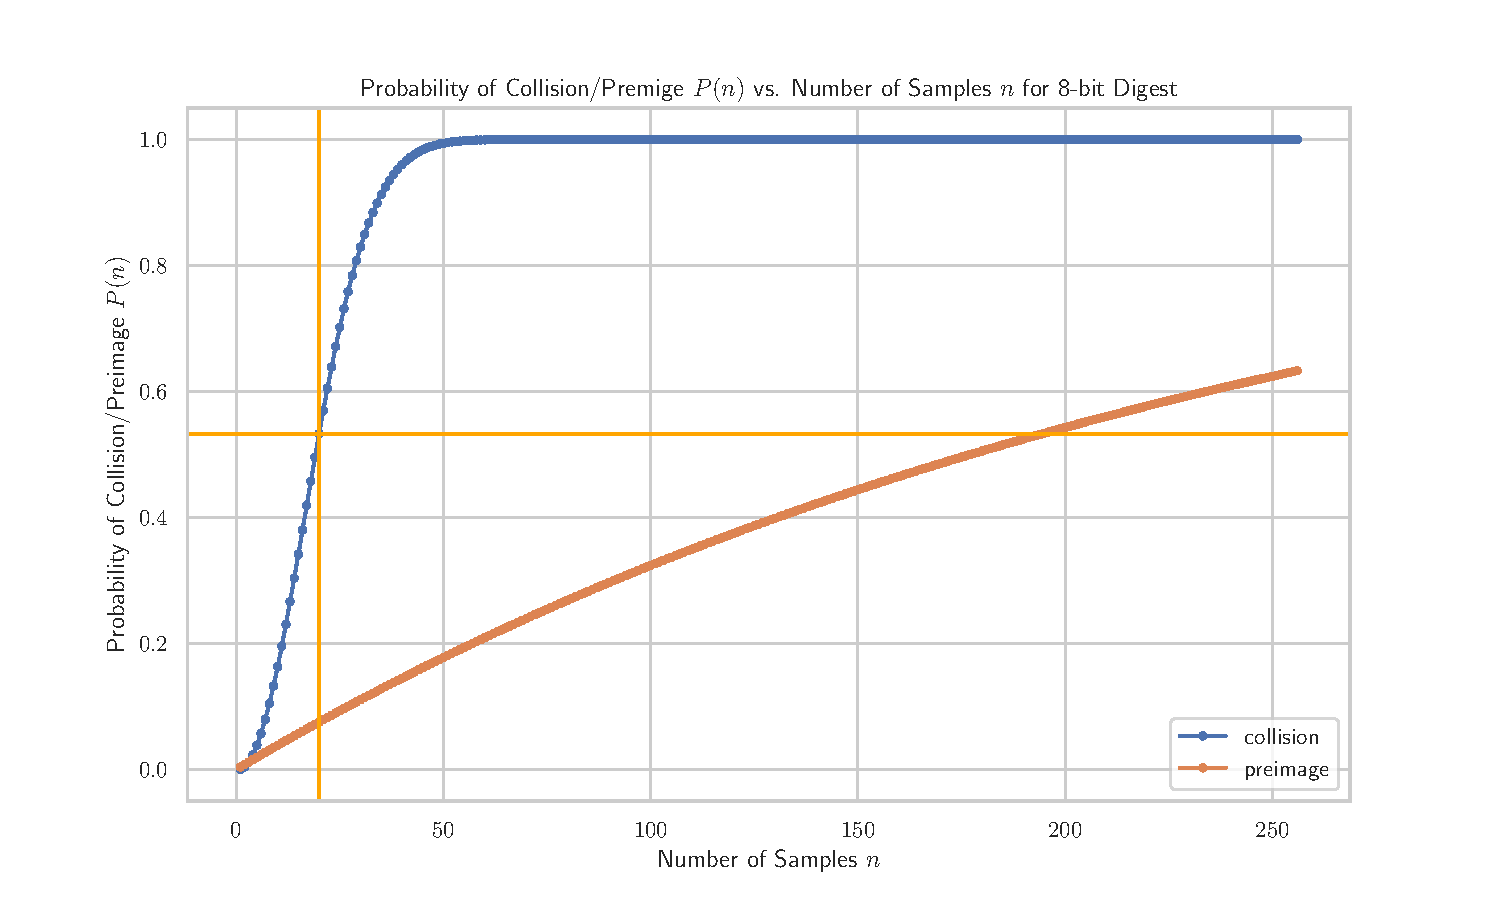
\includegraphics[width=\linewidth]{figure/birthday-paradox.pdf}
\captionsetup{width=.8\linewidth} 
\caption[Birthday Paradox with 8 Bits]{For a sequence of uniformly random draws of 8 bit numbers probability of at least one collision/preimage after $n$ draws $P(n)$ is compared to $n$. The orange cross-hair marks $P(20)$.}
\label{fig:birthday-paradox-8bits}
\end{figure}

It turns out that after only about $3.3\times10^{14}$ 96 bit \nonce s the probability of a collision reaches 50\%. While this is still a large number, if a protocol used a widely shared secret key $k$, and there were many (say billions) of clients using the same key, the chances of a \nonce reuse become high.
% Reusing a \nonce breaks confidentiality for \ac{AEAD} ciphers, and has even worse consequences for \ac{AES}-\ac{GCM}.

% [ ] \cite{aesgcm-security} attacker's advantage

\subsubsection{Nonce Brittleness}
\label{sec:nonce-brittleness}

Reuse of a $(\nonce,k)$ pair with AES-GCM destroys the confidentiality of the messages protected by that $(\nonce, k)$ pair. But for AES-GCM the consequence of $(\nonce,k)$ reuse is even worse, it allows an attacker to compute an underlying value $H$, which is used in all operations with key $k$ (even with a different \nonce). Possession of $H$ allows an attacker to forge messages, i.e. create cipher texts with valid authentication tags \cite[Section 5]{aesgcm-security}.

% [x] AES-GCM GHASH brittleness: using a (nonce,key) more than once allows an attacker to recover $H$ which means the attacker can forge messages forever (but does this mean the attacker can only forge when plaintext is empty?)

\section{HKDF}

The \acp{HKDF} described in RFC 5869 \citep{rfc5869hkdf} are used ubiquitously in the \ac{TLS} 1.3 protocol for the derivation of various traffic encpytion keys from the \ac{DHE} and/or \ac{PSK} secret.
Additionally \ac{HKDF} is proposed to be used for the \ac{ECH} \var{accept\_confirmation} 8 byte acceptance signal (see e.g. Section 7.2 of \cite{esni}).

A \ac{MAC} is a cryptographic verification of the integrity and/or authenticity of a message. The \ac{HMAC}, standardised in RFC 2104  \citep{rfc2104}, is a pattern for performing message authentication based on cryptographic hash functions, and the authentication is secured with a secret key.
A \ac{HMAC} scheme enables the calculation of the \ac{HMAC} digest over data with a secret key, and verification that the \ac{HMAC} matches the data and secret key.
A successful verificatoin of the \ac{HMAC} digest
implies that the data have not been tampered with (with high probability),
and that the \ac{HMAC} was calculated by someone who knows the secret key (with high probability).

The \ac{HKDF} scheme is all about using a \ac{HMAC} to transform some \ac{IKM} (some source of secret randomness/entropy)
into a set of (yes multiple!) pseudo-random cryptographic keys.

Key derivation is carried out in two stages: \var{HKDF-extract} and \var{HKDF-expand}.
If the \ac{IKM} is already cryptographically strong and of the appropriate length, e.g. if the \ac{IKM} is a random string of \var{Hash.length} bytes,
then the \var{HKDF-extract} stage can be safely skipped and the \ac{IKM}
can be transformed
directly into a sequence of pseudorandom keys using successive applications of the \var{HKDF-expand} function.
It is possible, however, that the input keying material may be too long to be directly used in the \var{HKDF-expand} function, or it may not be cryptographically suitable, e.g. the \ac{DH} value $g^{xy}$ is not uniformly random and therefore not suitable as a \ac{PRK} for the \var{HKDF-Expand} step.
So long as the \ac{IKM} contains sufficient entropy (read randomness), we can extract an appropriately long, uniformly (pseudo)random key from the \ac{IKM} by applying the \var{HKDF-extract} function.
For simplicity, when protocols use the extract-then-expand pattern, one can decide to always apply the \var{HKDF-Extract} stage, even if it is not always cryptographically necessary.

The \var{HKDF-Extract} function (the first step in the HKDF pattern) takes as input a salt (a non-secret random value) and the \ac{IKM} to produce a \ac{PRK}.
The salt is optional and is set to all zeros if not provided to the function, but is highly recommended in RFC 5869 Section 3.1.
Ideally the salt should be a random string,
and must have length equal to the length of the output of the underlying hash function used.
The second step is the \var{HKDF-Expand} function
which takes as input a \ac{PRK},
an optional information string (termed the label in \ac{TLS} 1.3),
and the desired length of the output,
to produce the \ac{OKM}.

The \var{HKDF-Extract} function is implemented as
\begin{verbatim}
HKDF-Extract(salt, IKM) = HMAC-Hash(salt, IKM)
\end{verbatim} where the salt is being used as the `key' for the \var{HMAC-Hash} (but it does not have to be secret)
and the \ac{IKM} is the `input message' of the \var{HMAC-Hash} function.
This means that the \ac{IKM} can have arbitrary length. The \ac{OKM} is generated recursively as \[T(n) = \text{\var{HMAC-Hash}}(\text{\var{PRK}}, \text{\var{concatenate}}(T(n-1), \text{\var{info}}, n))\], \[\text{\var{OKM}}=\text{\var{concatenate}}(T(1),T(2),\ldots)\]
but where $T(0)$ is an empty string.
This recursive pattern means that the \ac{OKM} can be very long.
The info parameter in \var{HKDF-Expand} can be used to bind the \ac{OKM} to particular contexts, e.g. in \ac{TLS} 1.3 the client-to-server and server-to-client encryption keys are generated with different info parameters, i.e. each key is unidirectional. 

\section{HPKE}
The basic mechanism of \ac{ECH} is to encrypt the \ac{ECHI} with a randomly generated secret symmetric key, and then encrypt the symmetric key using the public key of the ECH server.

This pattern of encryption-to-a-public-key has been standardised by the \ac{IETF} as \ac{HPKE} in RFC 9180 \citep{rfc9180hpke},
and \ac{ECH} uses \ac{HPKE} ciphersuites exclusively
for \ac{CH} encryption.

A \ac{HPKE} suite consists of three components, the \ac{KEM} for sending the shared secret,
the \ac{HKDF} for deriving unidirectional keys,
the \ac{AEAD} for encrypting the data.
\ac{DH} and \ac{EC}\ac{DH} are both families of key exchange methods that can be used to implement a \ac{KEM}.

\section{ The Diffie-Hellman Key Exchange }
The \ac{DH} key exchange protocol \citep{diffie-hellman-1976} allows two parties, Alice and Bob, to establish a secret shared key
while communicating over a public channel.
Variants and evolutions of the \ac{DH} key exchange protocol, in particular (\ac{EC})\ac{DHE},
are fundamental to how \ac{TLS} works.

A \ac{DH} key exchange involves Alice sending a \var{key\_share} to Bob, and Bob sending a \var{key\_share} to Alice. Both parties combine the two \var{key\_share}s in order to derive a shared secret which an eavesdropper cannot derive.

The original \ac{DH} key exchange was based on the
`apparent difficulty of computing logarithms over a finite field $GF(q)$ with a prime number $q$ of elements' \cite[p. 8]{diffie-hellman-1976}.
A finite field (a.k.a. Galois field), has a finite number of elements on which addition and multiplication are defined such that an additive inverse exists for all
elements and a multiplicative inverse exists for every nonzero element.
The integers with modular arithmetic modulo a prime number give us a finite field.

The \ac{DH} key exchange on finite field $GF(q)$ works as follows.
Alice and Bob each generate a secret independent random number $X_a$ and $X_b$ chosen uniformly from ${1,2,\dots,q-1}$.
Alice and Bob agree on a public value $g$, and each compute another public value $Y_i=g^{X_i}\mod q$.
Alice acquires $Y_b$ from Bob over an public channel, and vice versa.
% The original \ac{DH} description does not specify how Bob authenticates ownership of $Y_b$.
Alice and Bobs' shared secret is defined as $K_{ab}=g^{X_aX_b}\mod q$.
Alice computes this as $Y_b^{X_a}\mod q$ which is equivalent to Bob's $Y_a^{X_b}\mod q$.
Thus, Alice and Bob now each posses the shared secret $K_{ab}$.

When attacking \ac{DH} passively we observe $g$, $q$, $Y_a$, and $Y_b$.
We know that $Y_a=g^{X_a}\mod q$, and therefore that
\begin{equation}
\label{discrete-log-problem}
X_a=\log_g Y_a \mod q
\end{equation}
but it is computationally expensive to solve for $X_a$.
Equation~\ref{discrete-log-problem} is known as the discrete-log problem.
If a practical algorithm were discovered to solve the discrete-log problem efficiently then the \ac{DH} key exchange would be rendered ineffective.

Algorithms for solving the discrete-log problem do of course exist, so in order to use \ac{DH} securely in practice we have to choose a large enough $q$ such that computing the discrete-log becomes excessively expensive.
Unfortunately, choosing a large $q$ also entails a higher computational overhead for the benevolent parties, Alice and Bob.
Because of the mathematical relationship between the public and private values in \ac{PKC} it is generally the case that larger keys are required for \ac{PKC} than for symmetric cryptography in order to achieve the same security.

\subsection{DHE}
A problem with static \ac{DH} is that it is not forward secret. This means
that if one of the private keys is compromised then all past communications
based on the two \ac{DH} key pairs are compromised.
To combat this \ac{DHE} is a variant of \ac{DH} in which both public/private key pairs
are generated fresh for each connection. This means the security of each connection is more independent of the security of all past and future connections, i.e. compromising
the key of one connection does not necessarily compromise any other connection.
The \ac{TLS} 1.3 only allows ephemeral key exchanges. The only case in which \ac{TLS} 1.3 does not provide forward secrecy is when using an external \ac{PSK}.

\subsection{ECDHE}
\ac{EC}\ac{DHE} is a family of key exchange methods based on the mathematics of \acp{EC}
rather than finite fields.
For example, the Curve25519 crypto system is based on the elliptic curve $E$ defined by
$y^2=x^3+486662x^2+x$ and uses the Galois field $\mathbf{F}_p$ with prime number $p=2^{255}-19$.
Elliptic curve cryptography is based on a special definition for the addition
of two points on an elliptic curve $E$.
Say $P$ is on the curve $E$; $P\in E$,
then our special addition operation entails that $P+\ldots+P=kP\in E$. 
The difficulty of breaking elliptic curve cryptography is then based on
the computational complexity of finding $k$ given $Q$ and $P$ where $Q=kP$,
i.e. solving the elliptic curve discrete log problem.

\ac{X25519} has several desirable properties,
including the fact that for \ac{X25519} as a \ac{KEM} the \var{enc} (encapsulated shared secret) is a 32 byte value,
and all possible 32 byte values are valid \var{enc}s.
While it may be possible to distinguish between a long stream of \var{enc} values compared to a long stream of uniformly random 32 byte values,
the number of values needed to make this distinction would be large.
Our designs for \ac{SECH} 3 will make the assumption that
distinguishing between an \ac{X25519} \var{enc} and a truly random
value is hard enough such that detection is computationally infeasible

\section{TLS 1.3}
A \ac{TLS} 1.3 connection is initiated by the client's \ac{CH} message, which (usually)
contains an (\ac{EC})\ac{DHE} \var{key\_share}.
The server responds with its \var{key\_share} in the \ac{SH} followed by the first flight of encrypted messages: \ac{tlsEE}, \ac{tlsC}, \ac{CV}, and \ac{tlsF}.
After constructing the \ac{SH} the server can compute the server handshake traffic secret using \ac{HKDF}. The authentication messages \ac{tlsEE}, \ac{tlsC}, \ac{CV}, \ac{tlsF}, are all encrypted under \ac{AEAD} using this secret.

Upon receipt of the \ac{SH} the client also has enough information to construct the handshake secrets, and thus to decrypt the incoming authentication messages.
The client finally constructs the \ac{tlsF} message which contains a \ac{MAC} digesting the entire transcript of messages up to that point.

Since both parties verify each others \ac{tlsF} message, they are assured that the agreed keys and parameters have not been tampered with by a \ac{MITM}.

The flow described above is just one of various possible flows.
This flow involves just one full round-trip (one flight of messages from the client, one from the server) before the client can start sending application data.
The server can start sending messages after the third flight has been processed.

\subsection{Early Data}
\ac{TLS} 1.3 also permits application data in the first flight of client messages (called 0\ac{RTT} data),
but the protection of the `early data' is weaker,
in particular 0\ac{RTT} data is not protected against replays.
If the server processes the `early data' and passes it to the application
before the handshake has completed, then the application
may be processing maliciously replayed data (see Appendix~E of \cite{esni}).
Early data could potentially provide cover for an \ac{SECH} payload in the first flight.

\subsection{The \var{HelloRetryRequest} Message Type}
With TLS 1.3 the server can (hopefully in an overwhelming majority of cases) generate the application traffic key after processing just one flight of messages from the client. This is possible because the client `guesses' an (\ac{EC})\ac{DHE} curve/group and sends an appropriate \var{key\_share} in the \ac{CH} (in fact the client may send multiple \var{key\_share}s for multiple curves/groups to increase the probability that the server will support at least one of those cipher suites).
However, if the client guesses wrong and sends a \var{key\_share} for a curve/group not supported by the server,
then the server should respond with a message that informs the client as to which curves/groups are supported.
This subsequent message is called the \ac{HRR}.

The \ac{HRR} message format is designed to look almost identical to the \ac{SH} message for compatibility with hardened \ac{TLS} 1.2 middleboxes that fail to correctly ignore new message types for the first server message.
From the perspective of a middlebox
that is unaware of \ac{TLS} 1.3
the \ac{HRR} is treated just like a \ac{SH},
but the client can distinguish between \ac{HRR} and \ac{SH} based on a special value in the \var{random} field of the message.

\begin{listing}[hb]
    \centering
    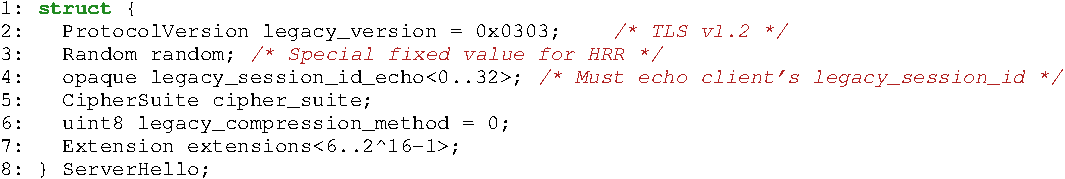
\includegraphics[width=\linewidth]{figure/ServerHello-struct.pdf}
    \captionsetup{width=.8\linewidth} 
    \caption[\ac{SH} and \ac{HRR} Structures]{The structure of the \ac{SH} message, which is the same as the structure of \ac{HRR}, repeated from Section 4.1.3 of \cite{esni} using the presentation syntax defined by same.}
    \label{lst:server-hello-struct}
\end{listing}

The use of the special constant value in the \var{random} field of the \ac{HRR} has implications for the design of the \ac{ECH} protocol.
In the happy case when the server accepts the first \ac{CH}
(it supports the curves/groups for the \var{key\_share} etc.),
and when the server also accepts \ac{ECH}, then the last 8 octets of the \ac{SH}\var{.random} are filled with a special ECH acceptance signal.
But, in the case where \ac{HRR} is necessary and \ac{ECH} is accepted
the last 8 octets of the \ac{HRR}\var{.random}
are not available because they are used to distinguish that the message is a \ac{HRR} and not a \ac{SH}.
Instead, in the case of \ac{HRR} {\em and} \ac{ECH} acceptance
the \ac{ECH} 8 byte acceptance signal is put in the
\var{ECHClientHello.payload} field of an \var{encrypted\_client\_hello} extension
(as described in Section 7.2.1 of \cite{esni}).
Using a distinct extension to deliver an acceptance signal is not stealthy, and hence cannot be adopted for \ac{SECH}.


\subsection{Tickets and Session Resumption}

A TLS 1.3 server can issue tickets to clients after successful completion of a handshake.
These tickets allow a client to initiate new \ac{TLS} 1.3
sessions with the client and achieve server authentication
with fewer messages (no \ac{tlsC} nor \ac{CV}).

% TODO repetition
The motivation for the \ac{TLS} 1.3 ticket system
comes from the typical behaviour of web browsers when loading and rendering web pages.
Many contemporary web pages rely on a large number of resources to be loaded from the server.
With the \ac{TLS} ticket system it is typical for a \ac{HTTPS} server
to issue several tickets (e.g. 6 or more) for every successful handshake.
This means that when a web browser is loading a web page it can first complete a full handshake,
and then open several more TLS connections to the server concurrently
in order to load subsequent resources with lower latency/bandwidth (e.g. images, videos, JavaScript files).

% [ ] Details of tickets as specified by TLS 1.3 RFC. \var{psk\_binder}, \var{NewSessionTicket} message type, what happens when multiple servers have authority on the server's certificate?

% [ ] the \var{pre\_shared\_key} extension
The structure of the \var{pre\_shared\_key} extension as defined in Section 4.2.11 of \cite{esni} is repeated in Listing \ref{lst:psk-struct}.
When the client offers \var{pre\_shared\_key} it contains a list of (\var{identity}, \var{binder}) pairs,
and if the server accepts \ac{PSK}-based key establishment it sends back just the index of the selected \var{identity}.
The \var{pre\_shared\_key} extension is exceptional in that it
"MUST be the last extension in the \ac{CH}" (\citet[Section 4.2]{esni}).
This restriction makes implementation of the \var{binders} slightly easier because each binder in \var{binders} is a \ac{HMAC} incorporating the entire \ac{CH} up to but excluding the list of \var{binders} themselves.

% The \var{PskIdentity} structure has an opaque \var{identity} field of between $1$ and $2^{16}-1$ bytes, which is plenty of room for stealthily sending encrypted data.

\begin{listing}
    \centering
    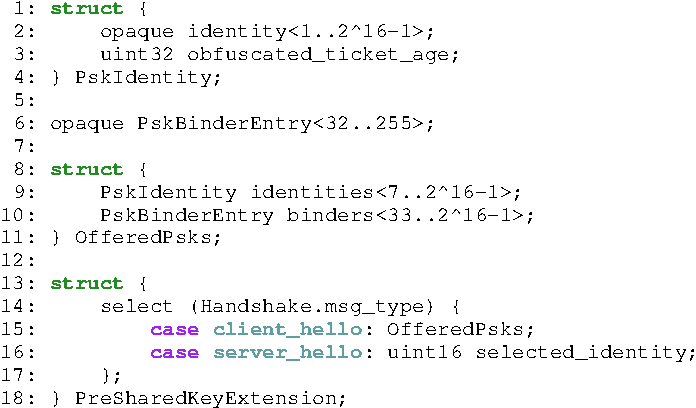
\includegraphics[width=.8\linewidth]{figure/pre_shared_key.pdf}
    \captionsetup{width=.8\linewidth} 
    \caption[Structures for the \var{pre\_shared\_key} extension]{TLS 1.3 presentation language representations of the structures used for the \var{pre\_shared\_key} extension.}
    \label{lst:psk-struct}
\end{listing}

The \ac{PSK} system has the potential for use as stealthy cover,
but in this work we pursue a design that instead uses \ac{PSK}s as way
of bootstrapping or distributing access to an \ac{SECH} server.

% [ ] Stateful/stateless cookies.

% [ ] Notes about how tickets are typically used in reality. Notes about any strict restrictions on the ticket behaviour in TLS 1.3 RFC.

% [ ] Introduce idea of using tickets to distribute access to an SECH server (will this be a way to distribute a symmetric key, or can the ticket allow a one-time connection that does not require the symmetric key?).

\subsection{ECH}
Above we described some
of the properties of \ac{ECH}
and the history of its development.
Here we take a closer look
at how it works and note
aspects that can and can not be carried over to an \ac{SECH} design.

\subsubsection{\var{ECHConfig}}
The \var{ECHConfig} is a public value containing a public key and other parameters
which an \ac{ECH} client needs in order to offer \ac{ECH}.

% ECHConfig structure and fields
\cite{esni} define (in Section 4) just one version (identified by the hextet \var{0xFE0D}) of the \var{ECHConfig}, but  the structure is defined in a way that will compatibly allow future versions.
The interesting part of the \var{ECHConfig} is the \var{ECHConfigContents} which has four fields,
the \var{key\_config}, the \var{maximum\_name\_length}, the \var{public\_name}, and \var{extensions}.
The \var{key\_config} contains the \var{public\_key} needed by a client to encrypt the \ac{CHI} under \ac{HPKE}.
As well as the \var{public\_key} the \var{key\_config} has a \var{config\_id},
a \ac{KEM} ID (\var{kem\_id}) and a list of \ac{HPKE} symmetric cipher suites supported by the \var{ECHConfig}.
The \var{config\_id} is ``A one-byte identifier for the given \ac{HPKE} [public] key''.

% hard to send config\_id stealthily
When a client offers \ac{ECH} it sends the \var{config\_id} of the public key used to encrypt the ClientHelloInner.
This \var{config\_id} means that the server only has to attempt decryption of the \ac{CHI} once,
which is essential for a scalable deployment of \ac{ECH},
supporting convenient regular config rotation.
In the case of a stealthy \ac{ECH} variant, however, transmitting a \var{config\_id} stealthily in the first flight of messages from the client (without permitting an attacker to detect the \ac{SECH} \var{config\_id}) is a challenge.
Our designs below facilitate multiple \ac{SECH} configs via trial decryption, which is expensive for the server.
For this reason we recommend against servers enabling multiple \ac{SECH} keys at one time.

For a \ac{TLS} connection the client just needs the servername and IP address to access the server,
but for \ac{ECH} the client additionally needs the public key of the \ac{ECH} backend server.
The \var{ECHConfig} will typically be distributed using \ac{DNS} alongside the server \ac{IP} address,
which means that the \ac{ECH} backend server will be advertising its own existence to users and censors alike.
But other ways of distributing \ac{ECH} configurations
such as having the \var{ECHconfig} pre-configured in the client, are also permissible.

Since the \ac{ECH} protocol is not stealthy there is little harm done in advertising the existence of the \ac{ECH} backend server.
It would be possible for a powerful attacker to enumerate \ac{ECH} backend servers with high confidence using \ac{DPI}, traffic analysis, and active probing, even if the \var{ECHConfig}
were not advertised.

For \ac{SECH} we have an opportunity to hide
the existence of backend \ac{SECH} servers from attackers,
which may be particularly beneficial for censorship-circumvention use cases.
If the existence of the backend \ac{SECH} server can be hidden from potential censors then the anonymity set for \ac{SECH} connections becomes the entire set
of all \ac{TLS} 1.3 servers on the Internet,
creating a very strong incentive against over-blocking.


% CLIENT                            CF-SERVER                             BACKEND SERVER
% ClientHelloOuter
% +encrypted\_client\_hello
% --------------------------------------->
%                                          ClientHelloInner
%                                          ------------------------------->
%                                                               ServerHello
%                                                      +accept\_confirmation
%                                          <-------------------------------
%                              ServerHello
%                     +accept\_confirmation
% <---------------------------------------

\subsubsection{ECH acceptance}

The \ac{ECH} acceptance signal is embedded into the first message sent by the server,
whether the first message is an \ac{SH} or an \ac{HRR},
however the location of the message is different in the \ac{HRR}.
This difference is an unfortunate added complexity.
An alternative design might have had the \ac{ECH} acceptance signal always embedded in the \ac{SH}, whether or not a \ac{HRR} is issued.
One reason such a design is not acceptable for \ac{ECH}
is that the client needs to know whether the message it is processing was constructed by the client-facing server or the backend server,
including whether the \ac{HRR} was sent by the client-facing or backend server.
To prevent certain kinds of attacks and to minimize bandwidth,
\ac{ECH} is designed so that
the client can abort the connection as soon as possible
if \ac{ECH} is rejected.
This situation is depicted in Figure~\ref{fig:ech-reject-and-hrr}% TODO: this is not quite right

\includefigure{fig:ech-reject-and-hrr}{
    Sequence Diagram of \ac{ECH} Rejection and \ac{HRR}}
    {
    A sequence diagram for a session in which the client attempts \ac{ECH} but \ac{ECH} is rejected {\em and} the parameters of the \ac{CHO} aren't supported (hence \ac{HRR}).
    Since \ac{ECH} is rejected the client responds with a fatal \var{ech\_required} alert in compliance with Section~5 of \cite{esni}.}{figure/ech-reject-and-hrr.pdf}

% If the \ac{HRR} is constructed by the client-facing server (i.e. ECH was rejected),
% then the \ac{HRR} corresponds to the ClientHelloOuter,
% but if the \ac{HRR} was constructed by the backend server then it corresponds to the \ac{CHI}.
% In order for the client to construct a valid \ac{CH2} it needs to know which ClientHello message the HRR is rejecting.
% While it may have been possible for a client to infer from the HRR contents (without an ECH acceptance signal) which ClientHello message it corresponds to (e.g. by process of elimination on the supplied cipher suites in either CH), this approach would not be robust and would make extensions to the protocol more complicated yet. Also, without the ECH acceptance signal it may be more difficult to analyse the security properties of the protocol due to an increased number of possible states the client can be in after processing the HRR.
% Also, according to \cite{esni} when a client offers ECH but the server does not accept then the client must terminate the connection with a \var{ech\_required} alert, which is not encrypted and thus transparent to network observers. In order to reduce the amount of unnecessary traffic ECH is designed so that the client can decide whether to emit the terminal \var{ech\_required} alert upon receipt of first server message.
Conversely, a stealthy variant of \ac{ECH} should not conspicuously terminate the connection when \ac{SECH} is rejected,
but ought to either continue with the handshake, emit an inconspicuous abort message, or abort silently in order to conceal the fact that \ac{SECH} was attempted.

It turns out that to maintain stealth the \ac{SECH} acceptance signal
needs to be cryptographically stronger than the
relatively weak 8 byte \ac{ECH} signal.
In particular, a preimage of the \ac{SECH} acceptance signal
could be used to trigger a client reaction that reveals \ac{SECH} is being attempted.
We propose a 24 byte \ac{SECH} acceptance signal embedded in the \ac{SH}\var{.random}.
This means the signal has better preimage resistance
than the 16 byte \ac{AES}-\ac{GCM} verification tag, 
which is in widespread use in \ac{TLS}.
The reason to use only 24 bytes rather than all 32 is to leave room for the possibility of running both \ac{SECH} and \ac{ECH} over the same connection.


\section{Considering a stealthy variant of ECH}
\subsection{Finding cover in TLS 1.3}
\label{sec:sech-cover-constraints}
We can potentially use any parts of the TLS 1.3 \ac{CH} message that look (or are) random,
as stealthy cover.
However, the quality of the cover depends on
various factors,
such as whether the field is necessary (i.e. always present in the client/server's first flight of messages),
whether the size or structure of the field
is implementation dependent,
and whether the semantics of the field can be used
to mount an attack that destroys stealth.

For our purposes we are looking for cover that does not depend
on the use of \ac{GREASE},
and which are essential to regular \ac{TLS} 1.3.
If we were to rely on a field which
is not necessary to regular \ac{TLS},
such as the \ac{PSK} or \ac{HRR}\var{.cookie}
then a censor could block all
connections containing that field to thwart \ac{SECH}.

Our conclusion is that the \var{random}
and \var{legacy\_session\_id} are the only parts of the client's first flight
of messages providing high quality stealthy cover that does not need to be \ac{GREASE}'d.
For the \ac{SH} the only high quality field is the 32 byte \var{random}.

\subsubsection{The \var{random}}
The \ac{CH}\var{.random} contains 32 random bytes, the purpose of which is to
ensure freshness of both the \ac{AEAD} symmetric keys
and the server's \ac{CV} message,
in order to prevent replay attacks.
The \ac{CH}\var{.random} provides high quality cover,
but using non-random values in its place could impact the security of the handshake.
We conjecture that it is cryptographically sound
to replace the \ac{CH}\var{.random} with ciphertext
since the ciphertext will be just as unpredictable as a random value from the perspective of an attacker.
However, it is beyond the scope of this project to
provide a formal or mechanistic attestation of this.
In \ac{TLS} 1.3 the \ac{CH2}\var{.random} must match the \ac{CH}\var{.random} if it exists. This means the \var{random} does not provide cover for a second encryption in the \ac{CH2}.


\subsubsection{The \var{legacy\_session\_id}}
The \ac{CH}\var{.legacy\_session\_id} also consists of 32 random bytes.
Its purpose
is to maintain compatibility with misbehaving
middleboxes.
It is essentially an example of the \ac{GREASE}
technique.
This field offers the highest quality cover because it is always present and plays no particular
role in the cryptographic negotiation.
The \var{legacy\_session\_id} is in fact intended to make \ac{TLS} 1.3 `look like' an earlier version of \ac{TLS},
and in our design we will use it to make \ac{SECH} `look like' \ac{TLS} 1.3.

Again the \varlegacysessionid{}
must be identical in the \ac{CH2},
so it offers no cover for a second encryption in the case of an \ac{HRR}.

\subsubsection{PSK}
Clients may send an arbitrary number of \acp{PSK}
identities in their \ac{CH}.
These identities can, for example, be self-encrypted ciphertexts created by the server
in a previous session.
Alongside each \ac{PSK} there must be a \var{binder},
which is a \ac{MAC} binding the use of the \ac{PSK} to the current session as well
as the session in which the \ac{PSK} was created.
Both the  \var{identities} field and \var{binders} field
have potential to be used as cover for \ac{SECH},
with the one caveat that the \ac{PSK} extension is not always present
in a \ac{CH}.
Relying on the \ac{PSK} for cover thus reveals a small amount of information
to an attacker about whether or not \ac{SECH} is being run.
Also, the size of the \ac{PSK} extension fields will vary between different
implementations and configurations,
meaning some empirical research would be needed in each deployment
in order to use the \ac{PSK} as cover in a way that does not stick relative
to the environment.

For these reasons we are pursuing in this work a design that does not use
the \ac{PSK} field as cover,
but we note that it remains a good option to pursue in future research,
in particular in order to expand the bandwidth of the \ac{SECH} payload.
\subsubsection{The Client's \var{key\_share}}
The \ac{CH}\var{.extensions.key\_share} has a field called \var{client\_shares} which is defined to contain between $0$ and $2^{16-1}$ bytes of data,
which can be parsed into a list of 0 or more key exchange public parameters.
The structure of this field depends on the set of
(\ac{EC})\ac{DHE} curves/groups listed in the \var{supported\_groups} extension.
The \var{supported\_groups} are listed in descending order of preference,
and the \var{client\_shares} must be listed in the same order.
To take a concrete example, let's say that
the first value in the \var{client\_shares} list
is an \ac{X25519} key share of length 32 bytes,
and the second is a \ac{p256} key share of 65 bytes.
The 32 bytes of the \ac{X25519} are hard to distinguish from random and thus provide good cover.
On the other hand the \ac{p256} has structure and would require
some finagling to be able to use it as cover stealthily.
Some values for the 65 bytes are not valid \ac{p256} key shares,
which an attacker could detect, so if a ciphertext took on one of those
impossible values, then an attacker could detect it.

If we use the \ac{X25519} key share as cover for ciphertext
then the key share value cannot be used for an actual key agreement,
since there is no associated private key with the fake public key (which is
actually ciphertext).
The problem with using the \ac{X25519} key share as cover is twofold:
1. it means we could not actually use the \ac{X25519} key exchange, and 2. it would expose us to an active attack that would destroy stealth.

That attack would work as follows. A client replaces the key share
value with ciphertext. The \ac{CH} is intercepted by an active attacker
who attempts to complete the key exchange using the client's fake key share.
The client does not have a private key and cannot compute the shared secret value
meaning the client cannot derive the handshake traffic secrets,
and in turn cannot decrypt the \ac{tlsEE} or \ac{tlsC} messages.
The attacker can leverage this to use the client's reaction as an oracle
to reveal that \ac{SECH} was attempted.
%The point at which the client should abort the handshake is when the attacker
%sends an invalid \ac{CV},
%since the attacker does not possess
%the private key associated with the \ac{tlsC}.
For example, if the attacker purposely sends a corrupted record the client should respond
with a \var{bad\_record\_mac} alert.
But with a properly formatted,
though invalid, \ac{CV} message the client
should respond with a \var{decrypt\_error} alert.
Without the handshake traffic secret the client is unable to determine
which response is appropriate,
so the client's reaction reveals that
the \ac{X25519} key share was fake.

For this reason we determine that the \var{key\_share} extension does
not provide cover for \ac{SECH} under an active-attacker threat model.

\subsubsection{Early Data}
The early data mechanism has the potential to provide a lot of
cover for \ac{SECH} payloads.
The lack of protection against replay for early data is worrying,
but replay protection could be handled in the \ac{SECH} design.
Similar to \acp{PSK}, though, the use of early data is situation and
implementation dependent,
so avoiding sticking out would require empirical analysis of the environment
and/or \ac{GREASE}ing.
We do not pursue the use of early data as cover in our designs,
but similar to \ac{PSK} this approach has good potential
for a design where the tradeoff is to maximise bandwidth rather than stealth.

\subsubsection{The Padding Extension}
The padding extensions \var{extension\_data} field `consists of an arbitrary number of zero bytes'.
This padding could be used as cover for SECH by using the length of the \var{extension\_data} as a piece
of data itself. Say we use padding as cover for some bits and set the maximum padding size to 15, then
the size of the padding encodes 4 bits of data:
\begin{verbatim}
Length   Payload
0     -> 0000
1     -> 0001
2     -> 0010
3     -> 0011
...
15    -> 1111
\end{verbatim}

The tradeoff between transmission size and stealthy bits is terrible here,
a padding extension of size 16 takes up 20 bytes (160 bits),
counting in the extension header, but offers only 4 covert bits.
Even worse, the total covert bits scales logarithmically with the maximum padding size.

The padding extension was introduced to solve issues with buggy implementations, and using
the padding extension for covert bits would require some engineering to ensure that the extension
could fulfill its original purpose.
Also, if the padding extension is used to encode covert bits (which may for instance be part of a cipher text),
then these covert bits will look uniformly random.
The padding extensions length is not usually random, so this would compromise stealth.


\subsubsection{Can we put a stealthy signal in the \var{HRR}?}

Let's consider a \ac{TLS} session in which a \ac{HRR} is triggered.
An easy way to achieve this practically is to set up a TLS 1.3 server which only supports an uncommon (\ac{EC})\ac{DHE} group such as P-384.
Most clients (including \var{openssl s\_client}) will not provide a P-384 \var{key\_share} by default in the ClientHello,
and the server will respond with a \ac{HRR} with a \var{key\_share} extension selecting \var{KeyShare.selected\_group = secp384r1}.
Note that the server-to-client \var{key\_share}
in a \ac{HRR} message contains only an indication of the type of key share the server supports,
but does not include a \var{KeyShareEntry}.
The total number of bytes in the \var{key\_share} extension in an \ac{HRR} message is 6: 2 for the extension length, 2 for the extension type, and 2 for the \var{SelectedGroup} field. Therefore, there is no room in the HRR server-to-client \var{key\_share} to embed a stealthy \ac{SECH} acceptance signal.
The other extension that will be present in the \ac{HRR} is the \var{supported\_versions}, which also has a length of 6 bytes, none of which can be manipulated stealthily.

Another option for sneaking an acceptance signal in the \ac{HRR}
could be to use the \var{cookie} extension as cover.
The cookie extension (identified by \var{0x002C})
allows the server to send arbitrary data
(of length $1$ to $2^{16}-1$ bytes) in either the \ac{HRR} or the \ac{SH}.
In accordance with \cite{rfc8446} when a client processes a cookie in an \ac{HRR}
it must echo the cookie extension exactly in the subsequent \ac{CH2} message.

Since the cookie extension is allowed in \var{HRR} messages and can contain opaque data it can be used to send a secret acceptance signal.
However, the cookie extension is not mandatory and may be used differently
(or not used at all) by different servers.
Thus, in order to successfully achieve a {\em stealthy} acceptance signal via the cookie, the extension would have to be manipulated in such a way that it does not stick out  when compared to normal \ac{TLS} traffic,
or \ac{TLS} traffic in the environment would have to be \ac{GREASE}'d.
For instance, the length of the cookie must not be an indicator of whether the cookie contains an acceptance signal.
Also, if the cookie were to be used for the acceptance signal a censor could block all connections that use \ac{HRR} cookies in order to thwart \ac{SECH}.

\cite{rfc8446} mention two purposes for the cookie extension;
\begin{enumerate}
    \item \ac{DoS} Mitigation: Forcing the client to echo back the cookie allows the server to verify that the client is `live', which increases the cost of (and thus mitigates) \ac{DoS} attacks.
    \item Offloading State: The cookie extension allows the server to `offload state' to the client, i.e. to ask the client to manage some data pertaining to the \ac{TLS} connection. By offloading state to the client the server can determine which messages belong to the same connection while running statelessly.
\end{enumerate}
If the \ac{HRR} cookie is used to hide an \ac{SECH} acceptance signal it interferes with these two capabilities.


% TODO repetition
For a design of a stealthy \ac{ECH} protocol we require that the \ac{SECH} acceptance signal also be stealthy.
For \ac{ECH} the acceptance signal is stealthy in the case that \ac{HRR} is skipped, but it is not stealthy when \ac{HRR} occurs.
To facilitate \ac{HRR} while performing \ac{SECH}
we would need a new mechanism to sneak the \ac{SECH} acceptance signal to the client.
One approach would be to delay the SECH acceptance signal until the true \ac{SH},
and put the \ac{SECH} acceptance signal
in the \var{ServerHello.random} field.
Another approach would be to use any other available random bytes in a typical \ac{HRR} and replace them with the acceptance signal.
As discussed there are no high-quality random bytes available
in the \ac{HRR}.
The \ac{HRR} cookie is not universally
present and can be used differently by different servers,
so leveraging the cookie without sticking out is difficult.

As we'll discuss in Section~\ref{sec:hrr-hijacking}
it turns out that facilitating the \ac{HRR} flow
for \ac{SECH} while maintaining stealth
is rather tricky due to \ac{HRR} hijacking.
For this reason in this work we have decided to drop the
goal of facilitating \ac{HRR} for \ac{SECH},
which means we only have to worry about
the \ac{SECH} acceptance signal
for the \ac{SH} message.



\subsection{Offering Both ECH and SECH}
While it is not immediately obvious that offering {\em both} \ac{ECH} and a stealthy \ac{SECH} variant could be beneficial there are some circumstances where offering both may in the future be necessary to protect privacy or facilitate censorship circumvention.
In particular the risk that \ac{ECH} will be blocked outright by some powerful censors (e.g. in China),
means that the convenience and enhanced privacy of regular ECH may be preferable in regions where ECH is not blocked,
but the stealthy alternative may be the only way to access the domain privately from regions where \ac{ECH} is blocked.
This is a clear case where servers may in future wish to offer both \ac{ECH} and \ac{SECH}.

But offering these two methods for accessing a resource privately
is an inherent increase in complexity of the overall system compared to a system that only offers {\em either}
\ac{ECH} {\em or} \ac{SECH}.
This increase in complexity increases the attack surface of the system,
there will be more branches of code on both the client and the server,
the cost of developing and deploying the additional code will be significant,
and the simultaneous co-operability of the two protocols presents new challenges to the design of each.

That the two protocols should co-operate also introduces an additional burden of analysis in terms of identifying and mitigating attacks against each of the protocols.
For all of these reasons there is a strong temptation to pursue developing versions of \ac{ECH} and \ac{SECH} that are designed {\em not} to co-operate with each other.

However, another pattern of argument relevant to most security protocols emphasises the importance of having a stand-by backup option to a widely deployed algorithm.
For instance, the most popular/widely-deployed \ac{AEAD} algorithm on the internet is AES-128-GCM,
but many software packages also support ChaCha20-Poly1305 because it could transpire
at any moment that AES-128-GCM has a fundamental flaw and needs to be replaced urgently.
This argument can also be applied to \ac{ECH} and \ac{SECH};
it would be wise to have both options ready, well-analysed, and deployed such that either one can be quickly disabled in case a fatal security flaw is discovered.

The above argument pertains to the simultaneous
deployment of \ac{ECH} and \ac{SECH} for a single domain,
but what about having versions of \ac{SECH} and \ac{ECH}
that facilitate the server accepting both \ac{ECH} and \ac{SECH} within a single TLS session?
Is there a motivation for such a design?
Consider, for example, an enterprise network in which the enterprise has control of client devices and is able to manage the list of trusted \ac{CA}s on each client device.
In such a case the enterprise network administrator will be able to mount a \ac{MITM} attack,
which would allow inspection of the TLS 1.3 application traffic as well as the \ac{CHI} if \ac{ECH} is being used.
There is motivation for network administrators to enforce such a situation for various reasons,
e.g. the enterprise network may be attempting to thwart phishing campaigns, and the risks of phishing campaigns can be mitigated by blocking traffic to suspicious or known malevolent servernames.
We can foresee a scenario, then,
where the network administrator decides to mount a \ac{MITM} attack in order to inspect the encrypted \ac{CH},
but no other part of the \ac{TLS} 1.3 encrypted traffic.
Let's imagine now we have a client trying to circumvent this \ac{MITM} attack.
If \ac{ECH} is available and used by default then it would be suspicious for the client not to use \ac{ECH}. However, the client may observe that using \ac{ECH}
to connect to \var{blocked.example.com} gets blocked,
and therefore will have to access \var{blocked.example.com} by some other means.
In such a case the client would benefit from the ability to make a `cover' \ac{ECH} connection request (to \var{allowed.example.com}, say)
and simultaneously an \ac{SECH} connection request to \var{blocked.example.com}.
To accommodate this scenario we would like for it to be possible to attempt \ac{ECH} and \ac{SECH} on the same connection.

One of the side-quests for this dissertation was to design \ac{SECH} such that it could run under \ac{ECH}.
We have not ended up pursuing this goal,
but some design decisions were made with
this goal in mind.

%It seems unlikely, however, that there would be much benefit from the server being able to accept both ECH and SECH, since the acceptance signal for ECH is sent in the same flight as the server certificate. If ECH and SECH are both accepted by the server, but with differing inner servernames (e.g. `ech.example.com` and `sech.example.com`), the server will have to select a certificate to send for the same flight of messages as the ECH acceptance signal. Possibly, it would be beneficial to the client to know that both were accepted, such that it can decide how to try to establish subsequent connections. 

% \subsection{Accepting SECH}

% The \ac{ECH} acceptance signal is necessary
% because the client continues the handshake differently (e.g. the Finished message is constructed with a transcript using the ClientHelloInner) when it detects a positive ECH \var{accept\_confirmation} signal from the server. The design of the ECH acceptance signal facilitates ECH split-mode, in which the backend server only processes one ClientHello (ClientHelloInner if the client-facing server accepts ECH, and ClientHelloOuter otherwise).

% [ ] The purpose of an SECH acceptance signal is to inform the client as early as possible whether or not the server is intending to use the inner or outer servername. It is sufficient to include only a positive signal (the server is accepting the SECH inner servername), and to infer that the outer servername will be used when the positive signal is absent.
%     - Detecting the length of the domain name

% [ ] must not be possible for an attacker to detect the length of the inner servername, merely knowing the length of the servername could leak the servername itself

\section{Threat Models and Attacks}

The \ac{TLS} threat model assumes all messages
are mediated by an active attacker,
and for the most part the \ac{ECH} threat model is the same.
However, there are active attacks that distinguish
\ac{ECH} \ac{GREASE} from proper \ac{ECH}.
In this work we pursue designs of a stealthy \ac{ECH}
which cannot be distinguished from a normal \ac{TLS} 1.3 connection,
even in the presence
of an active on-path adversary.

Various potential attacks against \ac{ECH}
have been discovered.
In Section~\ref{sec:active-attacks} we discuss
each of the active attacks highlighted by \cite{esni}
and explain our approach to mitigating them in the case of \ac{SECH}.

\subsection{Bleichenbacher Attacks \label{bleichenbacher-attack}}
\cite{bleichenbacher1998chosen} demonstrated how an attacker could reveal the \premastersecret{} of an \ac{SSL} 3.0 connection when the \premastersecret{} is protected with \ac{RSA} public key encryption.
The effectiveness of the attack varied according to the specifics of the implementation, in particular the granularity of information revealed by the server about why a handshake is aborted.
The method, which is based on informatoin leaked by the server about decryption failure or incorrect formatting of plaintexts, was quite easily generalised and variants of the attack have been repeatedly found.
Also, \cite{boeck2018robot} showed that variants of the attack were still effective against a broad set of Internet servers, despite years of research and effort spent trying to plug leaks in protocols and implementations.

\citeauthor{bleichenbacher1998chosen}'s (\citeyear{bleichenbacher1998chosen}) adaptive-chosen-ciphertext attack against \ac{RSA} when using  PKCS \#1 standard\footnote{\ac{PKCS}} concerns the situation where
the \ac{RSA} public key $n,e$ and the ciphertext $c$
are known to an attacker who wants to recover the secret message, $m=c^d\mod n$, or even
the \ac{RSA} secret key $d$.
In \ac{PKCS} \#1 the secret message is padded to the length of $n$, including a fixed prefix \var{0x00 0x02}.
By sending a malicious ciphertext $c'\equiv cs^e\mod n$, where $s$ is chosen adaptively, if a server reveals that the corresponding plaintext $m'=c'^d\mod n$ is correctly formatted, then the attacker knows the first two bytes of $m'$ are \var{0x00 0x02}.
By cleverly using this information in adapting successive choices of $s$ they find that for a 1024-bit modulus $n$ the expected number of oracle accesses needed to recover the secret message is about 1,000,000, which is reasonably low and hence enables practical attacks.

A primary goal of the \ac{SECH} protocol is to maintain confidentiality of the very fact that \ac{SECH} is being attempted\footnote{connection-level \ac{PC}},
and secondarily confidentiality of whether the server supports \ac{SECH}\footnote{channel-level \ac{PC}}.
Care must be taken, therefore, to ensure that responses (or lack of a response)
from a server,
such as an alert about encryption or formatting errors,
as well as the timing of those responses,
do not reveal information about whether:
1. the server supports \ac{SECH} at all, and
2. the client attempted \ac{SECH} in the given connection.
